\documentclass[letterpaper,11pt]{article}
\usepackage{graphicx}
\usepackage{listings}
\usepackage[super]{nth}
\usepackage[hyphens]{url}
\usepackage{hyperref}
\usepackage{amsmath}
\usepackage[makeroom]{cancel}
\usepackage[table]{xcolor}
\usepackage{comment}
\usepackage[space]{grffile}
\usepackage{csvsimple}
\usepackage{longtable}


\newcommand*{\srcPath}{../src}%

\lstset{
	basicstyle=\footnotesize,
	breaklines=true,
}

\begin{document}

\begin{titlepage}

\begin{center}

\Huge{Assignment 6}

\Large{CS 532:  Introduction to Web Science}

\Large{Spring 2018}

\Large{Chandrasekhar Reddy Muthyala}

\Large Finished on \today

\end{center}

\end{titlepage}

\newpage


% =================================
% First question
% =================================
\section*{1}

\subsection*{Question}

\begin{verbatim}
1.  Find 3 users who are closest to you in terms of age, 
gender, and occupation.  For each of those 3 users:

- what are their top 3 favorite films?
- bottom 3 least favorite films?

Based on the movie values in those 6 tables (3 users X (favorite +
least)), choose a user that you feel is most like you.  Feel 
free to note any outliers (e.g., "I mostly identify with user 123,
except I did not like ``Ghost'' at all").  

This user is the "substitute you".
\end{verbatim}

\clearpage
\subsection*{Answer}

Instead of manually picking out users from the data file provided, I wrote a script called \textbf{substituteMe.py} , shown in Listing \ref{lst:substituteMe}, which filters all users by the gender Male ``M'', the occupation of ``engineer'' and the age \textbf{24}. This script found multiple users with age 24. This left me with 3 users with the ids: 105, 268 and 69. 

To find their favorite and least favorite movies I added a function called \textit{findMoviesMerge}, which matched each user's review to their movie names and return the bottom and top movies sorted by their ratings, there were of course other movies with rating 5 but I simply took the top and bottom 3 provided. Their tables for top 3 films and bottom 3 films are shown in Table \ref{table:q1user1}, Table \ref{table:q1user2} and Table \ref{table:q1user3} respectively.



\begin{table}[htb]
\begin{tabular}{ | c | c | c | | c | c |}
\hline
\textbf{Rank} & \textbf{Top Favorite Movies} & \textbf{Rating} & \textbf{Least Favorite Movie} & \textbf{Rating} \\
\hline
1 &Gattaca (1997) & 5.0 & Devil's Advocate, The (1997) & 2.0 \\
\hline
2 &Titanic (1997)) & 5.0 & Saint, The (1997) & 2.0 \\
\hline
3 & L.A. Confidential (1997)& 5.0 & Mimic (1997) & 2.0 \\
\hline
\end{tabular}
\caption{User 105's favorite and least favorite movies}
\label{table:q1user1}
\end{table}

\begin{table}[htb]
\begin{tabular}{ | c | c | c | | c | c |}
\hline
\textbf{Rank} & \textbf{Top Favorite Movies} & \textbf{Rating} & \textbf{Least Favorite Movie} & \textbf{Rating} \\
\hline
1 & Aliens (1986) & 5.0 & Lawnmower Man, The (1992) & 1.0 \\
\hline
2 & Empire Strikes Back, The (1980) & 5.0 &Forget Paris (1995) & 1.0 \\
\hline
3 & Close Shave, A (1995) & 5.0 & Santa Clause, The (1994) & 1.0 \\
\hline
\end{tabular}
\caption{User 268's favorite and least favorite movies}
\label{table:q1user2}
\end{table}

\clearpage

\begin{table}[htb]
\begin{tabular}{ | c | c | c | | c | c |}
\hline
\textbf{Rank} & \textbf{Top Favorite Movies} & \textbf{Rating} & \textbf{Least Favorite Movie} & \textbf{Rating} \\
\hline
1 & Graduate, The (1967) & 5.0 &Devil's Own, The (1997) & 1.0 \\
\hline
2 & Scream (1996) & 5.0 &Peacemaker, The (1997) & 1.0 \\
\hline
3 & Empire Strikes Back, The (1980) & 5.0 &Saint, The (1997) & 2.0 \\
\hline
\end{tabular}
\caption{User 69's favorite and least favorite movies}
\label{table:q1user3}
\end{table}

 \lstinputlisting[frame=single,caption={Python script for determining closest 3 users},label=lst:substituteMe,captionpos=b,numbers=left,showspaces=false,showstringspaces=false,basicstyle=\footnotesize]{substituteMe.py}


\clearpage

% =================================
% Second question
% =================================

\section*{2}

\subsection*{Question}

\begin{verbatim}
2.  Which 5 users are most correlated to the substitute you? Which
5 users are least correlated (i.e., negative correlation)?
\end{verbatim}

\subsection*{Answer}

This question's answer relied heavily off the source code provided by the Programming Collective Intelligence book \cite{collectiveIntell}. I created a script called \textbf{pearsonCorrelation.py}, shown in Listing \ref{lst:correlateUsers}, which is also used later in questions 3 and 4. This question used the \textit{loadMovieLens}, which generated the user preferences, and \textit{findCorrelations} methods which finds the Sim Pearson correlation coefficient between ``substitute me,'' user 868, and every other user based on their preferences. The results of this are shown in Tables \ref{table:q2most} and \ref{table:q2least} and were saved to \textbf{correlatedUsers.txt} in my Github repository \cite{github}.

\begin{table}[htb]
\centering
\begin{tabular}{ | c | c |}
\hline
\textbf{User ID} & \textbf{Correlation} \\
\hline
853 & +1.0 \\
\hline
857 & +1.0 \\
\hline
898 & +1.0 \\ 
\hline
626 & +1.0 \\
\hline
724 & +1.0 \\
\hline
\end{tabular}
\caption{Most correlated users}
\label{table:q2most}
\end{table}

\begin{table}[htb]
\centering
\begin{tabular}{ | c | c | c | | c | c |}
\hline
\textbf{User ID} & \textbf{Correlation} \\
\hline
36 & -1.0 \\
\hline
404 & -1.0 \\
\hline
599 & -1.0 \\ 
\hline
628 & -1.0 \\
\hline
736 & -0.9045340337332909 \\
\hline
\end{tabular}
\caption{Least correlated users}
\label{table:q2least}
\end{table}

\clearpage

 \lstinputlisting[frame=single,caption={Python script utilizing Programming Collective Intelligence's code},label=lst:correlateUsers,captionpos=b,numbers=left,showspaces=false,showstringspaces=false,basicstyle=\footnotesize]{pearsonCorrelation.py}

\clearpage

% =================================
% 3rd question
% =================================

\section*{3}

\subsection*{Question}

\begin{verbatim}
3.  Compute ratings for all the films that the substitute you
have not seen.  Provide a list of the top 5 recommendations for films
that the substitute you should see.  Provide a list of the bottom
5 recommendations (i.e., films the substitute you is almost certain
to hate).
\end{verbatim}

\subsection*{Answer}

The answer for this question again relied heavily upon Programming Collective Intelligence's code since it provided the main method to solve this problem, the \textit{getRecommendations} method, and is shown in Listing \ref{lst:correlateUsers}. This again utilized the Sim Pearson correlation coefficient between users and found all the movies my substitute user, user 868, hasn't seen. After a final score was calculated these scores were normalized on a 1 to 5 scale and sorted in order. I took the lowest 5 movies and the top 5 movies, again with some being the same weight I simply took the top 5 it provided. These are shown in Table \ref{table:q3most} and \ref{table:q3least}.

I was taken aback when substitute me's second most recommended movie was ``Santa with Muscles (1996).'' He also apparently hates any kind of Amityville horror movie. I'll have to look into Saint of Fort Washington.

\begin{table}[htb]
\centering
\begin{tabular}{ | c | c | c |}
\hline
\textbf{Rank} & \textbf{Movie} & \textbf{Rating} \\
\hline
1 & Saint of Fort Washington, The (1993) & 5.0 \\
\hline
2 & Santa with Muscles (1996) & 5.0 \\
\hline
3 & Someone Else's America (1995) & 5.0 \\ 
\hline
4 & The Deadly Cure (1996) & 5.0 \\
\hline
5 & They Made Me a Criminal (1939) & 5.0 \\
\hline
\end{tabular}
\caption{Most recommended movies}
\label{table:q3most}
\end{table}

\begin{table}[htb]
\centering
\begin{tabular}{ | c | c | c |}
\hline
\textbf{Rank} & \textbf{Movie} & \textbf{Rating} \\
\hline
1 & 3 Ninjas: High Noon At Mega Mountain (1998) & 1.0 \\
\hline
2 & Amityville 1992: It's About Time (1992) & 1.0 \\
\hline
3 & Amityville: A New Generation (1993) & 1.0 \\ 
\hline
4 & Amityville: Dollhouse (1996) & 1.0 \\
\hline
5 & Babyfever (1994) & 1.0 \\
\hline
\end{tabular}
\caption{Least recommended movies}
\label{table:q3least}
\end{table}


\clearpage

% =================================
% 4th question
% =================================

\section*{4}

\subsection*{Question}

\begin{verbatim}
4.  Choose your (the real you, not the substitute you) favorite and
least favorite film from the data.  For each film, generate a list
of the top 5 most correlated and bottom 5 least correlated films.
Based on your knowledge of the resulting films, do you agree with
the results?  In other words, do you personally like / dislike
the resulting films?
\end{verbatim}

\subsection*{Answer}

When looked through the movie data I saw one of my favorite movies of all time, Citizen Kane (1941) because of the amazing cinematography for its time, I chose this film as my favorite. For me least favorite film I chose Mars Attacks! (1996). This question used the \textit{getRecommendations} method like in question 3, but this time I had to transform the preferences into a dictionary of movie as key and users as values. The method to do this was \textit{transformPrefs}, which was also provided by the Programming Collective Intelligence book \cite{collectiveIntell}. I then used the \textit{topMatches} method to get the bottom and top most correlated films. The results are shown in Tables \ref{table:q4most}, \ref{table:q4least}, \ref{table:q4most2} and \ref{table:q4least2} with the data saved to a files named \textbf{favoriteFilmCorrelation.txt} and \textbf{worstFilmCorrelation.txt} on my Github repository \cite{github}.

Its difficult to comment on the results of this problem as I have never seen any of the films in the tables below, aside from Free Willy, but not even that sequel number. I imagine that the films that least correlate with Citizen Kane also align with my dislikes after looking them up on the IMDB website. Aside from that, I really can't comment on the rest of the films.

\begin{table}[htb]
\centering
\begin{tabular}{ | c | c | c |}
\hline
\textbf{Rank} & \textbf{Movie} & \textbf{Correlation} \\
\hline
1 & Newton Boys, The (1998) & 1.0 \\
\hline
2 & Palmetto (1998) & 1.0 \\
\hline
3 & Savage Nights (Nuits fauves, Les) (1992) & 1.0 \\ 
\hline
4 & Wild America (1997) & 1.0 \\
\hline
5 & Heavy (1995) & 1.0 \\
\hline
\end{tabular}
\caption{Citizen Kane highest correlated movies}
\label{table:q4most}
\end{table}

\begin{table}[htb]
\centering
\begin{tabular}{ | c | c | c |}
\hline
\textbf{Rank} & \textbf{Movie} & \textbf{Correlation} \\
\hline
1 & Maya Lin: A Strong Clear Vision (1994) & -1.0 \\
\hline
2 & Free Willy 3: The Rescue (1997) & -1.0 \\
\hline
3 & Bad Girls (1994) & -1.0 \\ 
\hline
4 & Big Bully (1996) & -1.0 \\
\hline
5 & Colonel Chabert, Le (1994) & -1.0 \\
\hline
\end{tabular}
\caption{Citizen Kane least correlated movies}
\label{table:q4least}
\end{table}

%p2 of q4

\begin{table}[htb]
\centering
\begin{tabular}{ | c | c | c |}
\hline
\textbf{Rank} & \textbf{Movie} & \textbf{Correlation} \\
\hline
1 & Winter Guest, The (1997) & 1.0 \\
\hline
2 & Wonderful, Horrible Life of Leni Riefenstahl, The (1993) & 1.0 \\
\hline
3 & Wooden Man's Bride, The (Wu Kui) (1994) & 1.0 \\ 
\hline
4 & Kaspar Hauser (1993) & 1.0 \\
\hline
5 & Palmetto (1998) & 1.0 \\
\hline
\end{tabular}
\caption{Mars Attacks! highest correlated movies}
\label{table:q4most2}
\end{table}

\begin{table}[htb]
\centering
\begin{tabular}{ | c | c | c |}
\hline
\textbf{Rank} & \textbf{Movie} & \textbf{Correlation} \\
\hline
1 & Across the Sea of Time (1995) & -1.0 \\
\hline
2 & 8 Heads in a Duffel Bag (1997) & -1.0 \\
\hline
3 & Swan Princess, The (1994) & -1.0 \\ 
\hline
4 & 8 Seconds (1994) & -1.0 \\
\hline
5 & Aparajito (1956) & -1.0 \\
\hline
\end{tabular}
\caption{Mars Attacks! least correlated movies}
\label{table:q4least2}
\end{table}

\clearpage

% =================================
% 5th question
% =================================

\section*{5}

\subsection*{Question}

\begin{verbatim}
Extra credit (3 points)
5.  Rank the 1,682 movies according to the 1997/1998 MovieLense
data.  Now rank the same 1,682 movies according to todays (March
2016) IMDB data (break ties based on # of users, for example: 7.2
with 10,000 raters > 7.2 with 9,000 raters).

Draw a graph, where each dot is a film (i.e., 1,682 dots).  The
x-axis is the MovieLense ranking and the y-axis is today's IMDB
ranking.

What is Pearon's r for the two lists (along w/ the p-value)?  Assuming
the two user bases are interchangable (which might not be a good
assumption), what does this say about the attitudes about the films
after nearly 20 years?
\end{verbatim}

\subsection*{Answer}
For this problem I wrote a python program \textbf{getIMDBRating.py} to get the current  IMDB rating of movie lense data through OMDB API and storing all those corresponding IMDB rating and movie lense rating into \textbf{test.csv} file to draw correlation graph i wrote a another python program \textbf{scatterplot.py}.

\lstinputlisting[frame=single,caption={Python script for getting IMDB rating},label=lst:correlateUsers,captionpos=b,numbers=left,showspaces=false,showstringspaces=false,basicstyle=\footnotesize]{getIMDBRating.py}

\lstinputlisting[frame=single,caption={Python script for plotting correlation graph },label=lst:correlateUsers,captionpos=b,numbers=left,showspaces=false,showstringspaces=false,basicstyle=\footnotesize]{scatterplot.py}

\begin{figure}[h]
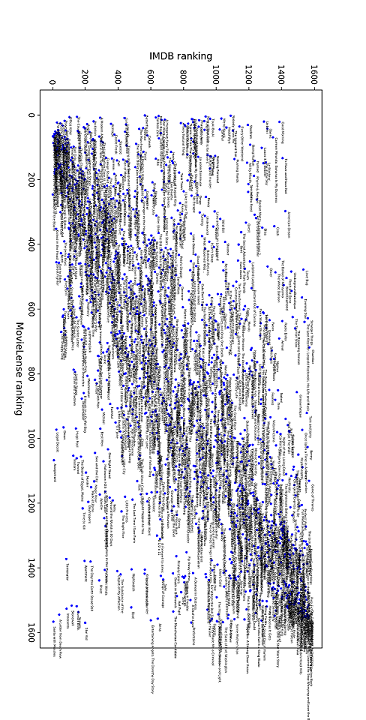
\includegraphics[scale=1.0]{dataset/Figure_1.png}
\caption{ MovieLense ranking VS today's IMDB
ranking}
\label{fig:q2histogram}
\end{figure}




\clearpage



% =================================
% Bibliography
% =================================

\begin{thebibliography}{9}

\bibitem{collectiveIntell}
Segaran, Toby. ``Programming Collective Intelligence''. O' Reilly, 2007. Web. 6 April 2017. \url{http://shop.oreilly.com/product/9780596529321.do}.
\end{thebibliography}

\end{document}